% !TEX encoding = IsoLatin2  % notwendige Zeile f"ur Mac-Benutzer (muss als Kommentar stehen); Windows-Benutzer k"onnen die Zeile l"oschen.

% LaTeX-Vorlage Version 3.1,  Juli 2011
% erstellt von Dr. Andreas Drauschke (andreas.drauschke@technikum-wien.at) und Dr. Susanne Teschl (susanne.teschl@technikum-wien.at)
% geringf"ugig adaptiert von Harald Stockinger (harald.stockinger@technikum-wien.at)

 
\documentclass[a4paper,bibtotoc,oneside]{scrbook} 
% F"ur kurze Arbeiten w"are auch die Dokumentklasse "scrartcl" ausreichend. In diesem Fall ist "section" die h"ochste Ebene ("chapter" gibt es dann nicht).
% \documentclass[a4paper,bibtotoc,oneside]{scrartcl}


% verlinkte Querverweise im pdf
\usepackage{hyperref}

% deutsche Anpassungen
\usepackage[ansinew]{inputenc}
\usepackage[T1]{fontenc}
\usepackage[ngerman]{babel}

% mathematische Symbole
\usepackage{amsmath,amssymb,amsfonts,amstext}

% Kopfzeilen frei gestaltbar
\usepackage{fancyhdr}
\lfoot[\fancyplain{}{}]{\fancyplain{}{}}
\rfoot[\fancyplain{}{}]{\fancyplain{}{}}
\cfoot[\fancyplain{}{\footnotesize\thepage}]{\fancyplain{}{\footnotesize\thepage}}
\lhead[\fancyplain{}{\footnotesize\nouppercase\leftmark}]{\fancyplain{}{}}
\chead{}
\rhead[\fancyplain{}{}]{\fancyplain{}{\footnotesize\nouppercase\sc\leftmark}} 

% Farben im Dokument m"oglich
\usepackage{color}

% Schriftart Helvetica
\usepackage{helvet}
\renewcommand{\familydefault}{cmss} 

% Graphiken einbinden: hier f"ur pdflatex
\usepackage[pdftex]{graphicx}

\usepackage{array}

% H"ohe und Breite des Textk"orpers etwas gr"osser definieren
\setlength{\textheight}{225mm}
\setlength{\textwidth}{1.05\textwidth}

% weniger Warnungen wegen "uberf"ullter Boxen
\tolerance = 9999
\sloppy

% Anpassung einiger "Uberschriften 
\renewcommand\figurename{Abbildung}
\renewcommand\tablename{Tabelle}

\begin{document}

% Kopf- und Fusszeilen initiieren
\pagestyle{fancy}

% Deckblatt:
\thispagestyle{empty}
\begin{picture}(0,0)
\color{white}\sffamily
\put(-101,-749){
\includegraphics[width=1.002\paperwidth, height=\paperheight]{BM_2011.pdf}}
\put(220,-670){
\includegraphics[width=0.5\textwidth]{FHTW_Logo_4c.pdf}}
\put(-30, -20){\bfseries\huge MASTER THESIS}
\put(-30,-50){\Large zur Erlangung des akademischen Grades}
\put(-30,-70){\Large \glqq Master of Science in Engineering\grqq}
% Titel des Studienganges einf"ugen:
\put(-30,-90){\Large im Studiengang XXX}
% Titel der Arbeit einf"ugen:
% Die Minipage wird gesetzt, damit auch mehrzeilige Titel m"oglich werden.
\put(-32,-180){
\begin{minipage}{14cm}
\bfseries\huge Arbeitstitel Arbeitstitel Arbeitstitel Arbeitstitel Arbeitstitel
\end{minipage}
}
% Name der Autorin/des Autors eingeben:
\put(-30,-270){\large Ausgef"uhrt von: Titel Vorname Name Titel}
% Personenkennzeichen der Autorin/des Autors eingeben:
\put(-30,-290){\large Personenkennzeichen: XXXXXXXXXX}
% Name der Begutachterinnen/der Begutachter eingeben:
\put(-30,-330){\large 1. BegutachterIn: Titel Vorname Name Titel}
\put(-30,-350){\large 2. BegutachterIn: Titel Vorname Name Titel}
\put(-30,-390){\large Wien, \today} % das Datum des letzten Kompilierens wird automatisch eingesetzt
\color{black}
\end{picture}

\newpage


\section*{Eidesstattliche Erkl"arung}\thispagestyle{empty}
\glqq Ich erkl"are hiermit an Eides statt, dass ich die vorliegende Arbeit selbst"andig angefertigt habe. 
Die aus fremden Quellen direkt oder indirekt "ubernommenen Gedanken sind als solche kenntlich gemacht. 
Die Arbeit wurde bisher weder in gleicher noch in "ahnlicher Form einer anderen Pr"ufungsbeh"orde vorgelegt
und auch noch nicht ver"offentlicht. Ich versichere, dass die abgegebene Version jener im Uploadtool entspricht.\grqq\\[5\baselineskip]
\rule{5cm}{0.2pt}\hfill\rule{5cm}{0.2pt}\\
\phantom{Datum }Ort, Datum\hfill Unterschrift\hspace{15mm}

\newpage



\section*{Kurzfassung}\thispagestyle{empty}
Text Text Text Text Text Text Text Text Text Text Text Text Text Text Text Text Text Text Text Text Text Text Text Text ...
\\ \vfill
% Bitte 3-5 deutsche Schlagw"orter eingeben, die die Arbeit charakterisieren:
\paragraph*{Schlagw"orter:} Schlagwort 1, Schlagwort 2, Schlagwort 3, Schlagwort 4, Schlagwort 5


\newpage

\section*{Abstract}\thispagestyle{empty}
Text Text Text Text Text Text Text Text Text Text Text Text Text Text Text Text Text Text Text Text Text Text Text Text ...
\\ \vfill
% Bitte 3-5 englische Keywords eingeben, die die Arbeit charakterisieren:
\paragraph*{Keywords:} Keyword 1, Keyword 2, Keyword 3, Keyword 4, Keyword 5
\newpage

\section*{Danksagung}\thispagestyle{empty}
Text Text Text Text Text Text Text Text Text Text Text Text Text Text Text Text Text Text Text Text Text Text Text Text ...
\newpage

\tableofcontents\thispagestyle{empty}
\newpage

\setcounter{page}{1}

% Falls die Kapitel"uberschriften zu lang f"ur die Kopfzeile oder das Inhaltsverzeichnis sind, so erzielt man
% dort Kurzformen der Kapitelbezeichnungen mittels:
% \chapter[Kurzform]{Lange "Uberschrift}
\chapter[Erstes Kapitel]{"Uberschrift des ersten Kapitels}

Text Text Text Text Text Text Text Text Text Text Text Text Text Text Text Text Text Text Text Text Text Text Text Text ...

Noch mehr text.

Und noch mehr TEXT:blabla

\section[Erster Abschnitt]{"Uberschrift des ersten Abschnitts}

Text Text Text Text Text Text Text Text Text Text Text Text Text Text Text Text Text Text Text Text Text Text Text Text ...

\subsection[Erster Unterabschnitt]{"Uberschrift des ersten Unterabschnitts}

Text Text Text Text Text Text Text Text Text Text Text Text Text Text Text Text Text Text Text Text Text Text Text Text ...

\subsubsection[Erster Unter-Unterabschnitt]{Und noch eine Ebene tiefer} 

Im Folgenden werden einige Beispiele f"ur h"aufig gebrauchte Anweisungen gegeben. Sie dienen als Einstiegshilfe in \LaTeX\ und 
nicht als starre Formatvorgaben.  
\\[2\baselineskip]
Hier wird auf Abbildung~\ref{Abb1} verwiesen. 
\begin{figure}[htbp]
\centering
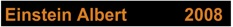
\includegraphics[width=75mm]{Buchruecken}
\caption[Beschriftung eines Buchr"uckens.]{Beispiel f"ur die Beschriftung eines Buchr"uckens.}\label{Abb1}
\end{figure}
Tabelle~\ref{Tab1} ist ein Beispiel daf"ur, wie eine Tabelle aussehen k"onnte.
\begin{table}[htbp]
\centering
\begin{tabular}{ | c | c | c | }\hline
{\bf Datum} & {\bf Thema} & {\bf Raum}\\ \hline
\hline
20. 08. 2008 & Graphentheorie & HS 3.13\\ \hline
01. 10. 2008 & Biomathematik & HS 1.05\\ \hline
\end{tabular}
\caption[Semesterplan "`Angewandte Mathematik"'.]{Beispiel f"ur einen Semesterplan "`Angewandte Mathematik"'.}\label{Tab1}
\end{table}

\noindent
Nun ein Beispiel f"ur eine abgesetzte Formel:
\begin{equation}
x =  - \frac{p}{2} \pm \sqrt{\left(\frac{p}{2}\right)^2 - q}.
\end{equation}
Und eine mehrzeilige Formel:
\begin{eqnarray}
f(t)&=& t^2 \label{For1},\\
g(t) &=& t-1.
\end{eqnarray}
Hier wird auf die Formel (\ref{For1}) verwiesen. \\

\noindent
So kann zum Beispiel ein \glqq Source-Code\grqq\  angegeben werden: 
\begin{verbatim}
for (i=1; i < 10; i++) {...} 
\end{verbatim}

\noindent
Hier ist ein Hyperlink auf die  \href{http://www.technikum-wien.at}{Homepage} der FH Technikum Wien. Email-Adressen k"onnen so verlinkt werden: \href{mailto:homer.simpson@springfield.com}{\texttt{homer.simpson@springfield.com}}\\

\noindent
In der Bibliothek der Fachhochschule Technikum Wien gibt es verschiedene einf"uhrende B"ucher zum Thema \glqq \LaTeX \grqq, zum Beispiel \cite{kop05}, \cite{wil06} oder \cite{mgb+05d} (deutsche Version) bzw. \cite{mgb+04e} (englische Version). Empfehlenswerte Skripten f"ur \LaTeX-Einsteiger sind z.B. \cite{mj00} und \cite{mj95}. Sie sind frei im Internet verf"ugbar.

% Literaturverzeichnis
% Das Literaturverzeichnis kann auch nach einem allf"alligen Anhang positiioniert werden (siehe "`Leitfaden f"ur Bachelor- und Diplomarbeiten"', Version 2.0, Abschnitt 2.9).

% M"oglichkeit 1: Erzeugung des Literaturverzeichnisses mit BibTeX:
% Die Quellen sind in der Datei *.bib (hier Literatur.bib) einzugeben. Danach muss diese Vorlage einmal geTeXt werden, dann BibTeX angewendet werden und 
% anschliessend nochmals zweimal geTeXt werden.
% Im Text erfolgt die Zitierung mit dem Anker-Schl"usselwort, z.B. \cite{kop05}.
\bibliographystyle{IEEEtran}
\bibliography{Literatur}

% M"oglichkeit 2: Erzeugung eines Literaturverzeichnisses ohne BibTeX:
%\begin{thebibliography}{99}
%\bibitem[kop05]{kop05}
%H.~Kopka, {\em LaTeX, Band 1: Einf"uhrung}, Pearson Studium, M"unchen, 3.~Auflage, 2005.
%\bibitem[knu98]{knu98}
%F.~Mittelbach, M.~Goossens, J.~Braams, D.~Carlisle, and Ch. Rowley, {\em The LaTeX Companion}, 
%Addison-Wesley, 2nd edition, 2004.
%\end{thebibliography}

% Abbildungsverzeichnis
\listoffigures
\addcontentsline{toc}{chapter}{Abbildungsverzeichnis} % f"ugt den Eintrag "Abbildungsverzeichnis" im Inhaltsverzeichnis hinzu
\newpage

% Tabellenverzeichnis
\listoftables 
\addcontentsline{toc}{chapter}{Tabellenverzeichnis} % f"ugt den Eintrag "Tabellenverzeichnis" im Inhaltsverzeichnis hinzu
\newpage

% Abk"urzungsverzeichnis
% Bei Verwendung der Dokumentklasse "scrartcl" ist der Befehlt \addchap{Abk"urzungsverzeichnis} durch 
% \addsec{Abk"urzungsverzeichnis} zu ersetzen
\addchap{Abk"urzungsverzeichnis}
\hspace{-17mm}\begin{tabular}{>{\raggedleft}p{0.2\linewidth} p{0.75\linewidth} p{0.1\linewidth}}
www & World Wide Web \\
URL & Uniform Resource Locator
\end{tabular}


% Anh"ange
\begin{appendix}
\chapter[Erster Anhang]{"Uberschrift des ersten Anhangs}

Text Text Text Text Text Text Text Text Text Text Text Text Text Text Text Text Text Text Text Text Text Text Text Text ...
 

\chapter[Zweiter Anhang]{"Uberschrift des zweiten Anhangs}

Text Text Text Text Text Text Text Text Text Text Text Text Text Text Text Text Text Text Text Text Text Text Text Text ...

\end{appendix}


\end{document}
